\documentclass{report}
\usepackage[T1]{fontenc}
\usepackage{color}
\usepackage{amssymb}
\usepackage{pdfpages}
\usepackage{amsmath}
\usepackage{eurosym}
\usepackage{graphicx}
\usepackage{textcomp}
\usepackage{listings}
\usepackage{epigraph}
<<<<<<< HEAD
\usepackage{longtable}
=======
>>>>>>> f70441dc9c662077ee37d70a107543de21584119
\usepackage{setspace}
\usepackage{array}
\usepackage{gensymb}
\usepackage{tikz}
\usepackage[some]{background}
\usepackage{geometry}
\usepackage[francais]{babel}


\begin{document}
\renewcommand{\contentsname}{Sommaire}
<<<<<<< HEAD
\renewcommand{\chaptername}{Part}
=======
\renewcommand{\chaptername}{Partie}
>>>>>>> f70441dc9c662077ee37d70a107543de21584119
\renewcommand{\thechapter}{\Roman{chapter}}

%\usepackage{lmodern}
%\usepackage{xspace}
%\usepackage{hyperref}

\definecolor{sup_strip_color}{rgb}{0.70,0.70,0.70}
\definecolor{inf_strip_color}{rgb}{0.00,0.00,0.00}

\DeclareFixedFont{\bigsf}{T1}{phv}{b}{n}{0.7cm}

\makeatletter                       
\def\printauthor{%                  
    {{\large \@author}}}              
\makeatother

\author{Zohour \textsc{Abouakil} ~\\ Sofia \textsc{Boutahar} ~\\ David \textsc{Courtinot} ~\\ Xiaowen \textsc{Ji} ~\\ Fabien \textsc{Sauce}}

\begin{titlepage}

\newgeometry{left=1cm,right=4cm}
\begin{tikzpicture}[overlay,remember picture]
% the black stripe with the title
\node[
  fill=inf_strip_color,
  anchor=north west,
  text width=\paperwidth,
  text height=2cm,
  text depth=2cm,
  inner xsep=1cm,
  font=\color{white}\bigsf 
  ] 
<<<<<<< HEAD
 at ([yshift=-2.5cm]current page.north west) (blackrect) {Plan de d\'{e}veloppement};
=======
 at ([yshift=-2.5cm]current page.north west) (blackrect) {Development plan};
>>>>>>> f70441dc9c662077ee37d70a107543de21584119
% the khaki stripe
\path[fill=sup_strip_color] 
  (blackrect.north west) rectangle ++(\paperwidth,2.5cm);
\end{tikzpicture}

\vspace*{4.5cm}

\noindent
\begin{minipage}{0.35\linewidth}
    \begin{flushright}
        \printauthor
    \end{flushright}
\end{minipage} \hspace{15pt}
%
\begin{minipage}{0.02\linewidth}
    \rule{1pt}{175pt}
\end{minipage} \hspace{-10pt}
%
\begin{minipage}{0.6\linewidth}
\vspace{5pt}
\newenvironment{test}{\begin{center}}{\end{center}}
\hspace{10pt}
\begin{minipage}{\linewidth} 
Recherche de motifs dans un code C++ \`{a} l'aide de la logique temporelle
\end{minipage}
\end{minipage}

\end{titlepage}
\restoregeometry
\tableofcontents
<<<<<<< HEAD

\chapter{Project description and objectives}
=======
\chapter{Project description and objectives test test}
>>>>>>> f70441dc9c662077ee37d70a107543de21584119

\section{Surroundings of the project}

\paragraph{}
\hspace{4mm}\textnormal{Le projet long \`{a} l'ENSEEIHT
	Organisation du projet}

\paragraph{}
\hspace{4mm}\textnormal{Le client c est qui ?? Les noms, leurs fonctions, les motivations du projet}

\paragraph{}
\hspace{4mm}\textnormal{Nos motivations -- pas sur}

\section{Project description}

\subsection{Main idea}

\subsection{Related technologies}

\vspace{4mm}
\begin{itemize}
\item Coccinelle\vspace{1mm}
\item Clang\vspace{1mm}
\end{itemize}

\subsection{Project parts}

\vspace{4mm}
\begin{itemize}
\item Parser\vspace{1mm}
\item CTL\vspace{1mm}
\item Model checking\vspace{1mm}
\end{itemize}

\subsection{To conclude}

\section{Final project}

\subsection{Define priorities}

\subsection{Deliverable documents}

\chapter{Project organization}

\section{Role definition}

\subsubsection{Project manager}

\paragraph{}
\hspace{4mm}\textnormal{}

\subsubsection{Quality manager}

\paragraph{}
\hspace{4mm}\textnormal{}

\subsubsection{Test manager}

\paragraph{}
\hspace{4mm}\textnormal{}

\subsubsection{Test manager}

\paragraph{}
\hspace{4mm}\textnormal{}

\subsubsection{Configuration manager}

\paragraph{}
\hspace{4mm}\textnormal{}

\subsubsection{Documentation manager}

\paragraph{}
\hspace{4mm}\textnormal{}

\subsubsection{Chain development}

\begin{center}
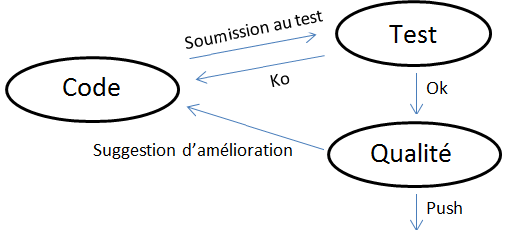
\includegraphics[scale=0.7]{data/cycle_qualite}
~\\~\\Figure II.1 - Sch\'{e}ma descriptif de la cha\^{i}ne de d\'{e}veloppement
\end{center}

<<<<<<< HEAD
\section{Development organization}
=======
\section{Development organisation}
>>>>>>> f70441dc9c662077ee37d70a107543de21584119

\paragraph{}
\hspace{4mm}\textnormal{To secure our evolution we can use :}

<<<<<<< HEAD
\subsection{Use of a software development framework : Scrum}

\paragraph{}
\hspace{4mm}\textnormal{}
=======
\subsection{Usage of Scrum method}

\paragraph{}
\hspace{4mm}\textnormal{We will try to use Scrum method, which is actually widely used, and 
recognised for its effectiveness. At first, we will define a 
\textit{product backlog} containing all desired functionalities in 
the final product. In fact, this report is also a part of \textit{product backlog}. 
Next, we will divide the project into three \textit{sprints} (which means 
iterations). A \textit{sprint backlog} is defined for each \textit{sprint}, 
including all we need to realise at the end of an iteration. Each 
\textit{sprint} lasts two weeks and lies in improve the software 
incrementally, so that it is close to \textit{product backlog}.}

\paragraph{}
\hspace{4mm}\textnormal{At the end of each \textit{sprint}, we will organise a meeting, in order to 
review the progress and propose improvements or modifications of planning,
 but in the process of a \textit{sprint}, we cannot modify the \textit{sprint backlog}. 
At last, each day starts with a \textit{scrum meeting}, on the meeting, each 
team member present his objective of the day and his actual difficulties.}
>>>>>>> f70441dc9c662077ee37d70a107543de21584119

\subsection{Team repartition approach}

\paragraph{}
<<<<<<< HEAD
\hspace{4mm}\textnormal{}

\section{Tasks organization}

\subsection{Tasks definition}

\subsection{Planning}

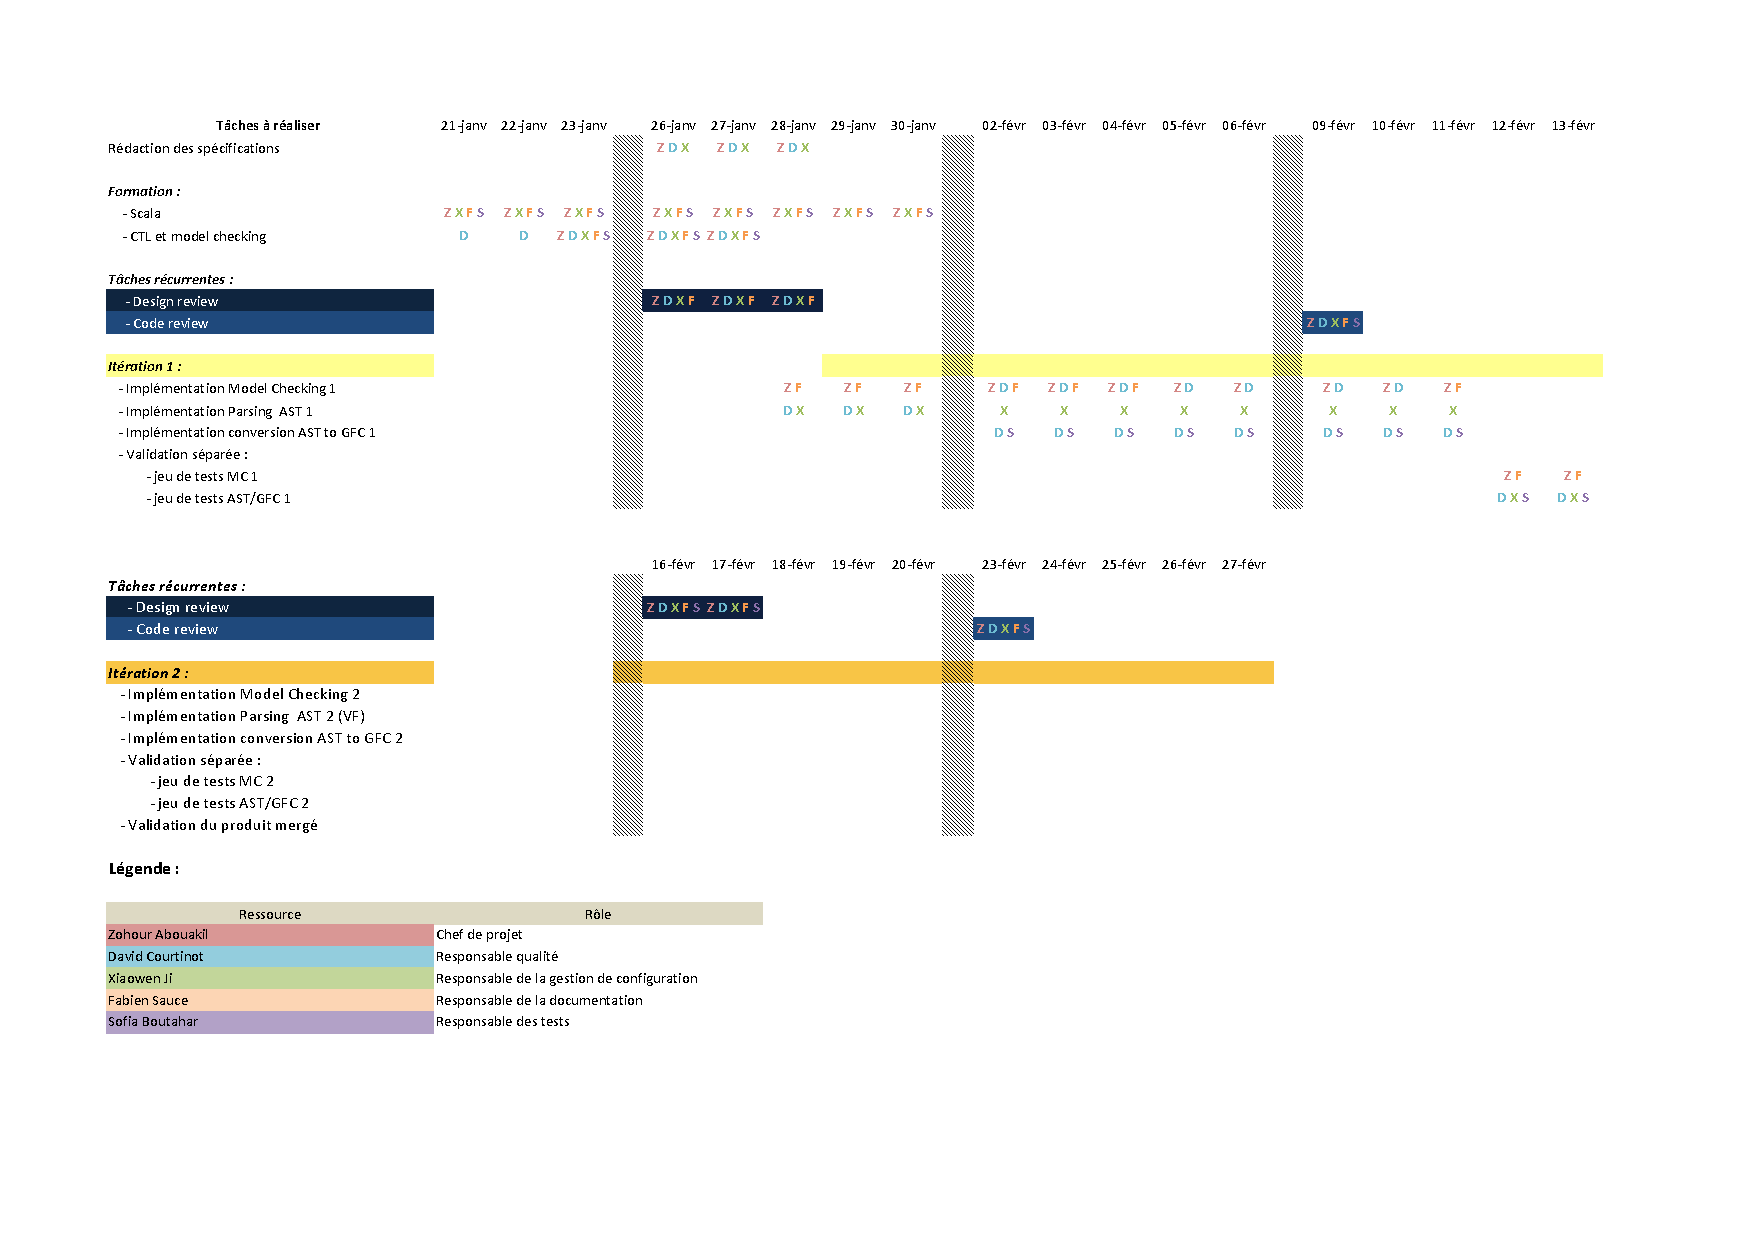
\includepdf[landscape=true,pages={1-2}]{data/planning.pdf}
\chapter{Risk management}

%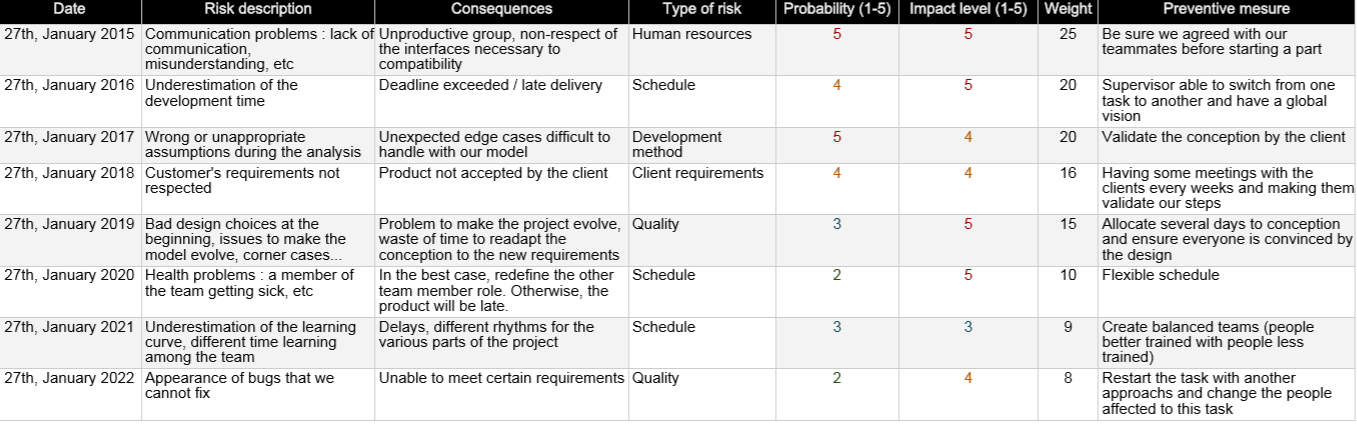
\includepdf[landscape=true,pages={1}]{data/risks.png}
\newgeometry{left=1.5cm,,right=1.5cm}
\begin{center}
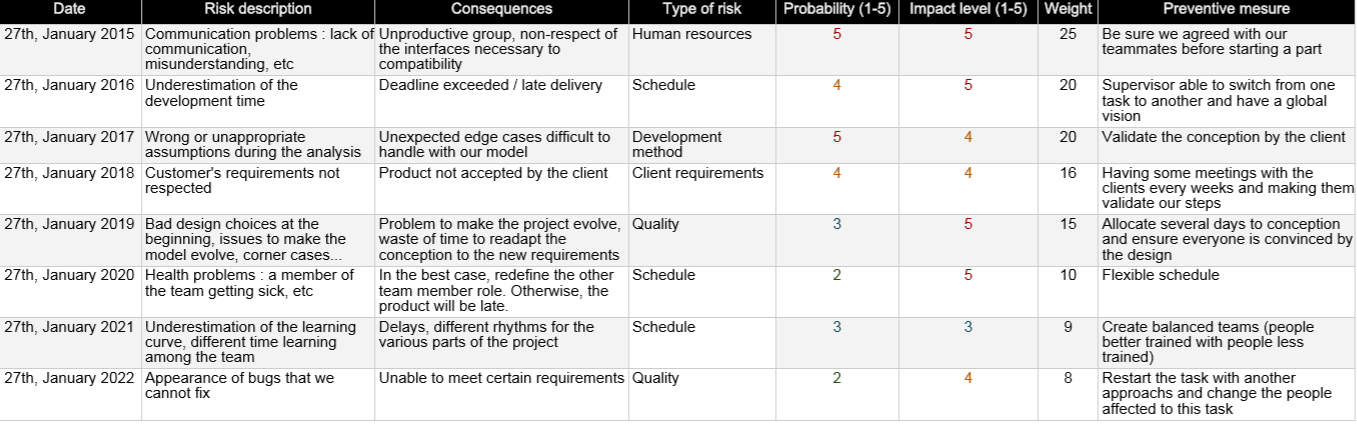
\includegraphics[scale=0.5]{data/risks.png}
~\\~\\Figure III.1 - Analyse des risques
\end{center}

=======
\hspace{4mm}\textnormal{We will use an approach inspired by the XP (extreme programming) method. 
In fact, we found it unnecessary that the team members work separately, 
and we found it excellent to work in pairs, in order to prevent errors and bias 
of the program structure, so that we can save times of testing and debugging. 
So four of us work in pairs and the last one works individually. The group 
will changes as the tasks are completed.}

\section{Tasks organisation}

\subsection{Tasks definition}

\paragraph{}
\hspace{4mm}\textnormal{Sprint 1 backlog:}

\vspace{4mm}
\begin{itemize}
\item AST parsing of procedure C++ code\vspace{1mm}
\item CFG conversion from parsed AST\vspace{1mm}
\item Model checking with simple properties\vspace{1mm}
\item \vspace{1mm}
\end{itemize}

\paragraph{}
\hspace{4mm}\textnormal{Sprint 2 backlog:}

\vspace{4mm}
\begin{itemize}
\item AST parsing of object oriented C++ code\vspace{1mm}
\item CFG conversion from parsed AST\vspace{1mm}
\item Model checking with simple criteria\vspace{1mm}
\item \vspace{1mm}
\end{itemize}

\paragraph{}
\hspace{4mm}\textnormal{Improved CFG conversion from parsed AST;
Model checking with complex criteria;}

\subsection{Planning}

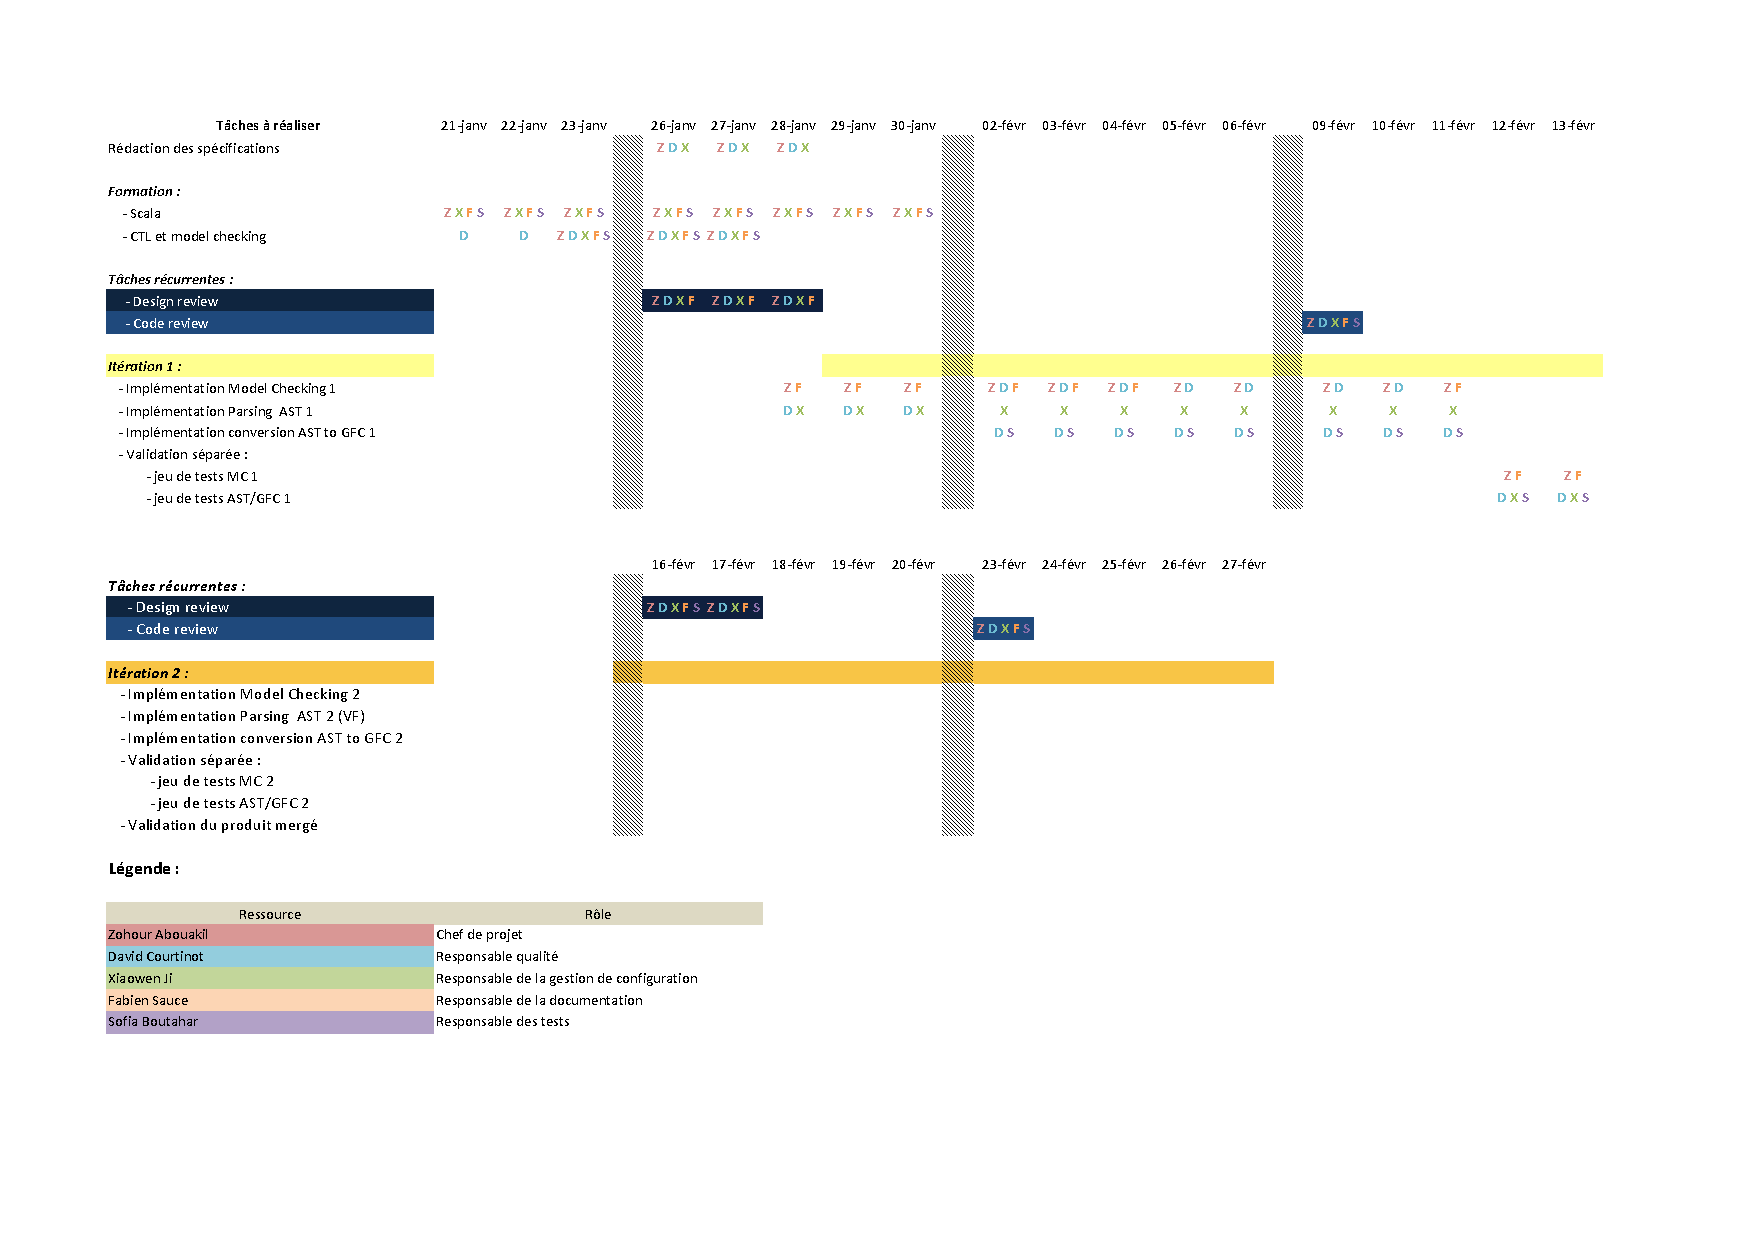
\includepdf[landscape=true,pages={1}]{data/planning.pdf}
\chapter{Risk management}

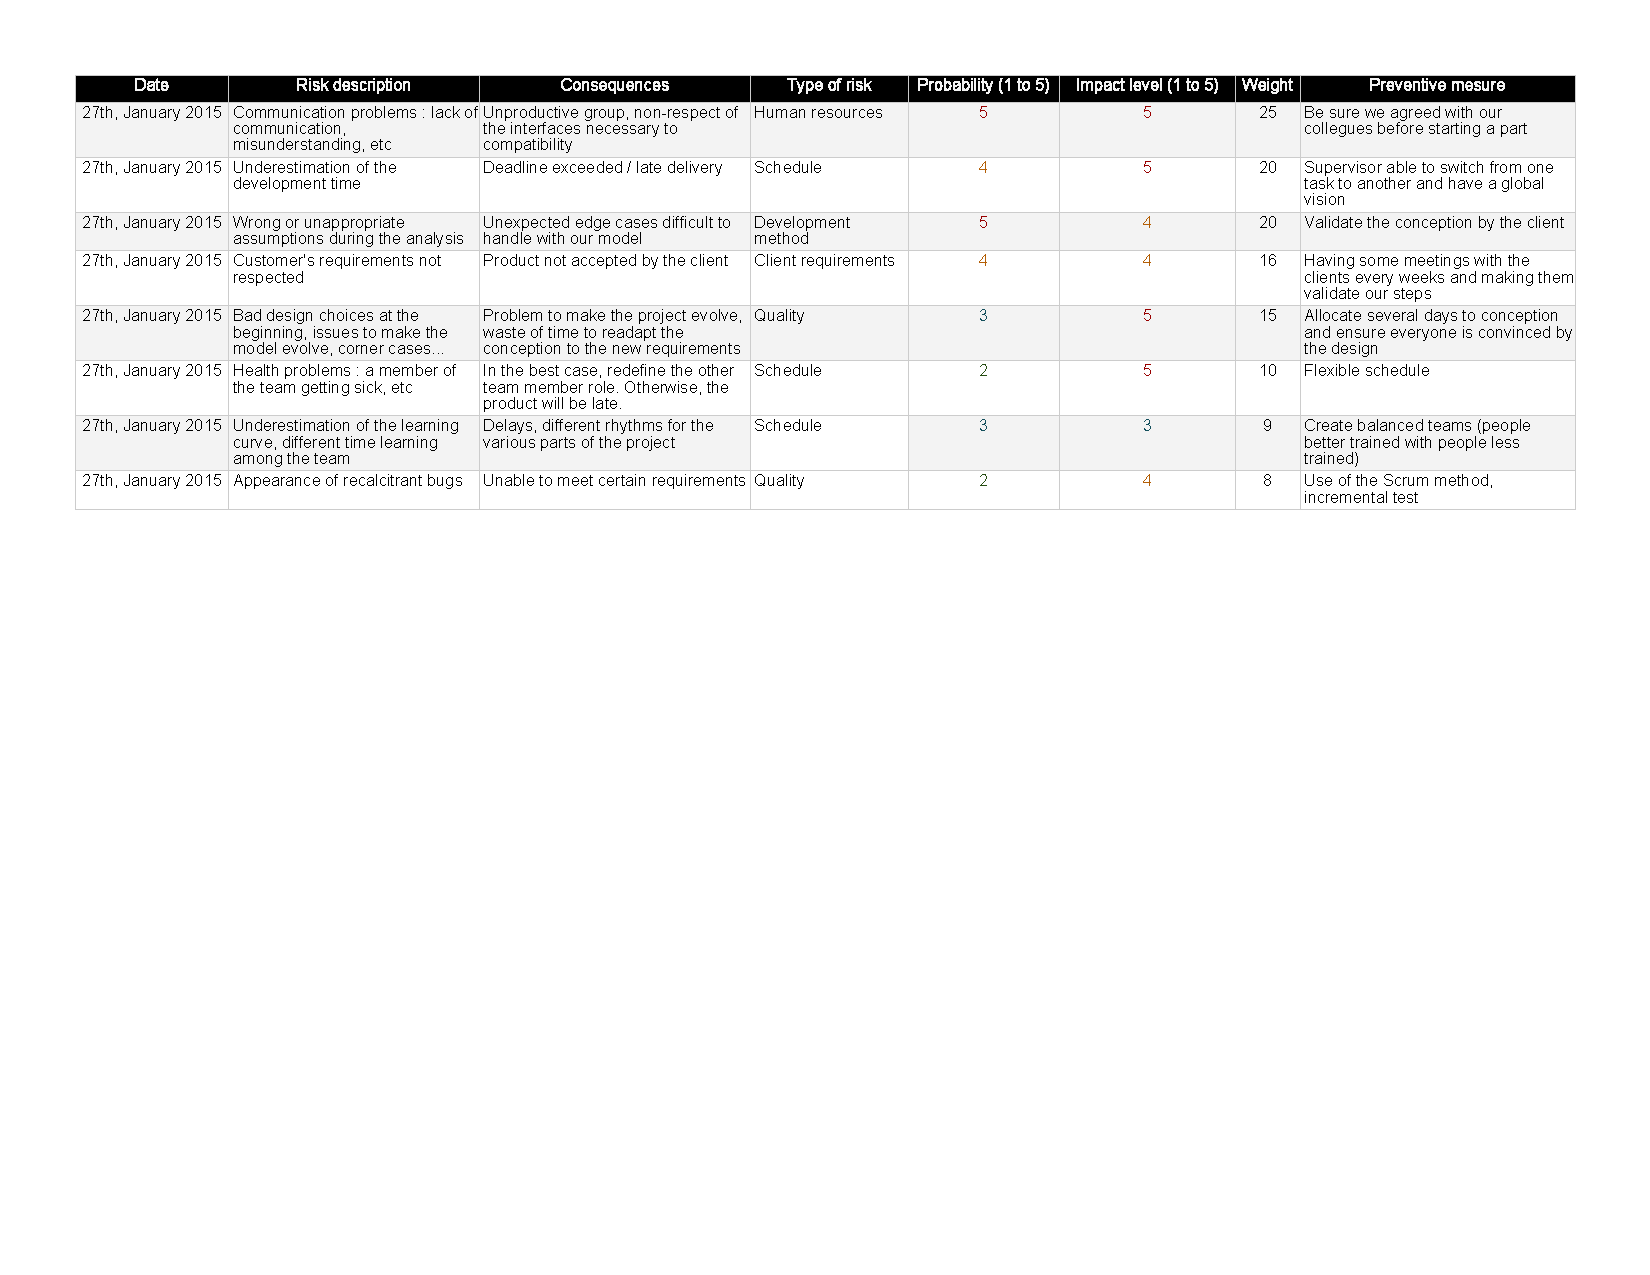
\includepdf[landscape=true,pages={1}]{data/risks.pdf}
>>>>>>> f70441dc9c662077ee37d70a107543de21584119
\chapter{Code management}

\section{Quality management}

\subsection{Automated coding style checks}

\paragraph{}
\hspace{4mm}\textnormal{For ensuring that our coding rules are respected and evaluate the quality of our sources, we have
used a tool called \textit{Scalastyle} that enables, using an easy-to-use xml configuration file, to check
some properties on a Scala code. Combined with a specific pulgin, this can be use to generate warnings or errors
<<<<<<< HEAD
in the IDE the developer is using. Our settings are the following :}

%\newgeometry{left=1.5cm,,right=1.5cm}
\renewcommand{\arraystretch}{1.2}
\begin{center}
\begin{longtable}{|l|l|l|}
\hline
\textbf{Rule} & \textbf{Description} & \textbf{Value}  \\
\hline
FileLengthChecker & \small{Check the number of lines in a file} & 1500  \\
\hline
FileLineLengthChecker & \small{Check the number of characters in a line} & 140 \\
\hline
FileTabChecker & \small{Check that there are no tabs in a file} & enabled \\
\hline
ClassNamesChecker & \small{Check that class names match a regular}  & \^ [A-Z][A-a-z]*\$ \\
& \small{expression} & \\
\hline
\small{ClassTypeParameterChecker} & \small{Checks that type parameter to a class matches a} & \^[A-Z\_]\$ \\
& regular expression & \\
\hline
FileTabChecker & \small{Check that there are no tabs in a file} & enabled \\
\hline
\small{CyclomaticComplexityChecker} & \small{Checks that the cyclomatic complexity of a method} & 12 \\
&  \small{does exceed a value} & \\
\hline
EmptyClassChecker & \small{If a class/trait has no members, the braces are} & enabled \\
&  \small{unnecessary} & \\
\hline
\small{EqualsHashCodeChecker} & \small{Check that if a class implements either equals} & enabled \\ 
 & \small{or hashCode, it should implement the other} & \\
\hline
MagicNumberChecker & \small{Checks for use of magic numbers instead of} & ignore = -1, 0, 1 \\
& \small{constants (safer)} & \\
\hline
MethodLengthChecker & \small{Checks that methods do not exceed a maximum} & 50 \\
& \small{length} & \\
\hline
MethodNamesChecker & \small{Check that method names match a regular} & \^[a-z][A-Za-z0-9]*(\_=)?\$ \\
\tiny{.} & \small{expression} & \\
\hline
\small{MultipleStringLiteralsChecker} & \small{Checks that a string literal does not appear} & allowed = 2 \\
& \small{multiple times} & \\
\hline
\small{NotImplementedErrorUsage} & \small{Checks that the code does not have ??? operators} & enabled \\
\hline
NullChecker & \small{Check that null is not used} & enabled \\
\hline
\small{NumberOfMethodsInTypeChecker} & \small{Check that a class/trait/object does not have too} & maxMethods = 30 \\
& \small{many methods} & \\
\hline
NumberOfTypesChecker & \small{Checks that there are not too many types} & maxTypes = 20 \\
& \small{declared in a file} & \\
\hline
ObjectNamesChecker & \small{Check that object names match a regular}  & \^[A-Z][A-Za-z]*\$ \\
& \small{expression} & \\
\hline
ParameterNumberChecker & \small{Maximum number of parameters for a method} & maxParameters = 5 \\
\hline
RedundantIfChecker & \small{Checks that if expressions are not redundant, ie} & enabled \\
& \small{easily replaced by a variant of the condition} &  \\
\hline
ScalaDocChecker & \small{Checks that the ScalaDoc on documentable}  & enabled \\
& \small{members is well-formed} & \\
\hline
\end{longtable} 
\end{center}
% \restoregeometry
\renewcommand{\arraystretch}{1}
=======
in the IDE the developer is using. Our settings can be found in appendix A.}

>>>>>>> f70441dc9c662077ee37d70a107543de21584119
\section{Test strategy}

\paragraph{}
\hspace{4mm}\textnormal{}

\section{Configuration management}

\paragraph{}
\hspace{4mm}\textnormal{}

\chapter{Appendices}

\end{document}
